\chapter{Herramientas utilizadas}
\label{cap:capitulo3}

El desarrollo de los 2 nuevos ejercicios de Robotics Academy han abarcado varios campos: programación, Docker, modelado y simulación de robots, ROS y ROS2, visión artificial, machine learning, desarrollo web... por lo que es necesario introducir y describir las herramientas y tecnologías utilizadas al lector.\\




% -- SECCIÓN C++
% ----------------
\section{C++}
\label{sec:c++}

C++ es un lenguaje de programación diseñado en 1979 por \textbf{Bjarne Stroustrup}. Deriva del lenguaje C, y destaca principalmente porque incorpora el paradigma de la \textbf{Programación Orientada a Objetos} (POO). Además, incorpora una novedosa librería que facilita el desarrollo de Software de calidad: \textbf{STL (Standard Template Library)}: vector, stack, map, etc. \cite{history_c++}\\

\begin{code}[H]
\begin{lstlisting}[language=C++]
#include <iostream>

int main(int argc, char ** argv)
{
	std::cout << "Hello World!\n";
	return 0;
}
\end{lstlisting}
\caption[Hola mundo en C++]{Hola mundo en C++}
\label{cod:holamundo_cplusplus}
\end{code}

\textbf{¿Cuál ha sido la utilidad de C++ en este proyecto?} La programación de un \textbf{plugin} que permite mover a una persona simulada en Gazebo \footnote{\textbf{Gazebo}: simulador robótico} con el teclado.\\




% -- SECCIÓN PYTHON
% -------------------
\section{Python}
\label{sec:python}

Python es un lenguaje de programación \textbf{interpretado} \footnote{\textbf{Interprete} (programación): programa informático que se encarga de ejecutar las instrucciones de otro programa sin compilación previa} que destaca por su legibilidad, facilidad y soportabilidad con el paradigma \textbf{POO}. Posee características particulares que lo diferencian de otros lenguajes de programación como puede ser el uso estricto de indentación en bloques de código, o incluso la capacidad de crear listas mezcladas de diferentes tipos de datos.\\

\begin{code}[H]
\begin{lstlisting}[language=Python]
print("Hola mundo")
\end{lstlisting}
\caption[Hola mundo en Python]{Hola mundo en Python}
\label{cod:holamundo_python}
\end{code}

\textbf{¿Cuál ha sido la utilidad de Python en este proyecto?} El desarrollo de la infraestructura interna que da soporte a los dos nuevos ejercicios de Robotics Academy, programación de nodos de ROS (más en la sección \ref{sec:ros}) y ficheros de lanzamiento, creación de los módulos HAL y GUI y desarollo de las soluciones de referencia de los ejercicios.\\




% -- SECCION ROS
% ----------------
\section{ROS (Robot Operating System)}
\label{sec:ros}
ROS (Robot Operating System) \cite{ROS} es un middleware \footnote{\textbf{Middleware}: software que se sitúa entre las aplicaciones y el sistema operativo} que ayuda a la programación de robots a través de varias \textbf{librerías} y \textbf{herramientas} desarrolladas por la comunidad de software libre. Entre las ayudas que proporciona este framework están la abstracción del hardware, controladores de dispositivos, herramientas de visualización (rviz) y geometría espacial (transformadas, tfs) entre otros.\\

El \textbf{funcionamiento} de ROS se basa en una arquitectura \textbf{cliente-servidor} centralizado donde un nodo principal se encarga del intercambio de mensajes entre otros nodos que forman la aplicación (remotos o locales), los cuales se comportan como \textbf{publicadores o suscriptores} del proceso de comunicación. El objetivo es dividir el software robótico en secciones o \textbf{nodos} que se encargan de realizar tareas específicas de manera \textbf{concurrente}: recogida de datos de la cámara, ejecución de una máquina de estados o árboles de comportamiento (Behavior Trees), recogida de las lecturas del láser, navegación, etc.\\

El intercambio de mensajes se realiza a través \textbf{topics}. Un nodo puede tener \textbf{publicadores}, \textbf{suscriptores} o ambos. Cuando un nodo publica un mensaje lo hace a través de un topic que gestiona el nodo maestro. Si otro nodo quiere leer ese mensaje tendrá que suscribirse al tópic correspondiente. Por ejemplo: en nuestro robot Turtlebot 2 podemos comandar velocidades enviando mensajes de tipo \textbf{geometry\_msgs.msg.Twist} a través del topic \textbf{/cmd\_vel}. En la figura se puede ver con más detalle \ref{fig:ros_master_comunicacion}\\

\begin{figure} [H]
  \begin{center}
    \includegraphics[width=15cm]{imagenes/ros_master_communication.png}
  \end{center}
  \caption{Comunicación del nodo Master con los nodos Intermedios (ROS)}
  \label{fig:ros_master_comunicación}
\end{figure}\

Desde un principio, ROS se ha ejecutado sobre sistemas operativos de tipo Unix (Ubuntu - principal), aunque han ido surgiendo versiones beta para otros SOs como Windows o MacOS X. La primera distribución de ROS salió en 2010 (ROS Box Turtle) y a partir de ahí han ido surgiendo nuevas distribuciones siendo la actual y estable ROS Noetic.\\

Las librerías que incorpora ROS estan desarrolladas en \textbf{C++} y \textbf{Python}. Con estos lenguajes de programación podemos desarrollar los nodos de los paquetes que tendrá nuestra aplicación. También incorpora un conjunto de comandos de \textbf{Shell} \footnote{\textbf{Shell}: Programa que toma entradas del usuario a través del teclado y pasa esos comandos al sistema operativo para realizar una función específica}. Para hacer tareas de depuración, creación, compilación, etc.\\

En 2016 surge ROS 2, nuevo framework basado en ROS que incorpora nuevas mejoras como la \textbf{calidad de servicio}, \textbf{lifecycle nodes} o \textbf{seguridad} (DDS) para asegurar la autenticación de los nodos y la integridad de los mensajes. Al igual que con ROS 1 ha tenido varias distribuciones siendo la primera \textbf{ROS Ardent}. La versión más reciente y estable es \textbf{ROS Foxy}, que es la que hemos usado en este proyecto.\\

Aprender ROS no es una tarea sencilla y requiere mucha dedicación y esfuerzo. Por lo tanto, el objetivo de Robotics Academy es proporcionar una interfaz de programación sencilla para programar robots sin necesidad de saber ROS. Es decir, el usuario tiene acceso a unas librerías HAL y GUI, las cuales usan por debajo nodos de ROS, y de esta manera, se puede centrar más en el desarrollo del algoritmo.\\

\textbf{¿Cuál ha sido la utilidad de ROS2 en este proyecto?}
\begin{itemize}
	\item Crear los ficheros \textbf{interfaces} (laser.py, motors.py, camera.py, ...) que se comunican con los topics necesarios para el control del robot Turtlebot 2 tanto real como simulado. Estos ficheros usan nodos con publicadores o suscriptores de distintos topics como /cmd\_vel, /scan, /odom o /raw\_image.
	\item Crear los \textbf{paquetes} de la simulación del hospital y la adaptación del Turtlebot 2 simulado.
	\item Incorporar de Github los paquetes de ROS 2 para controlar la base kobuki del robot real, y el láser RPLIDAR. Profundizaremos en el capítulo [\ref{cap:capitulo6}]
\end{itemize}

Durante la etapa de entrenamiento del TFG, usamos una modalidad para hacer unas primeras pruebas con el Robot Turtlebot 2 simulado de ROS Noetic en ROS 2. Para lograr esto, usamos \textbf{ROS Bridge} \footnote{\textbf{ROS Bridge}: \url{https://github.com/ros2/ros1_bridge}}. Se trata de un paquete que proporciona un puente de red que permite el intercambio de mensajes entre ROS 1 y ROS 2. De esta manera, podíamos lanzar una simulación en ROS 1 y ejecutar un programa en ROS 2 (el cual se comunica con los topics lanzados en el nodo maestro de ROS 1).\\




% -- GAZEBO
% -----------
\section{Gazebo}
\label{sec:gazebo}

Gazebo \cite{Gazebo} es un \textbf{simulador robótico} que nos permite integrar escenarios realistas con robos simulados para desarrollar y probar algoritmos. Gazebo surgió en 2002 en la Universidad del Sur de California. En 2009 un ingeniero superior de investigación integró \textbf{ROS} y el \textbf{robot PR2} en Gazebo.\\

Gazebo presenta estas características relevantes para nuestro proyecto:
\begin{itemize}
	\item Usa \textbf{motores de físicas} de alto rendimiento incluido Bullet, OGRE, Simbody y DART
	\item Puede simular \textbf{sensores} y su \textbf{ruido} característico para asemejarlo con el mundo real (RPLIDAR, camaras Kinect, sensores de contacto).
	\item Se puede programar \textbf{plugins} para incorporar nuevas características. Gazebo incorpora su propia API para ello.
	\item Muchos robots tienen soporte en Gazebo como PR2, Pioneer2 DX,  o \textbf{Turtlebot 2} y 3. También permite construir robots propios usando \textbf{SDF} (o URDF).
\end{itemize}

\begin{figure} [H]
  \begin{center}
    \includegraphics[width=10cm]{imagenes/simulacion-gazebo.png}
  \end{center}
  \caption{Simulador Gazebo (demostración)}
  \label{fig:simulador_gazebo}
\end{figure}\

\textbf{¿Cuál ha sido la utilidad de Gazebo en este proyecto?} Incorporar un escenario proporcionado por AWS que simula un hospital e integrar el robot simulado Turtlebot 2 (sensores incluidos) adaptado para ROS 2 Foxy. El nuevo ejercicio \textbf{Follow Person} simulado hace uso de dicho simulador.\\




% -- SECCION URDF
% -----------------
\section{URDF}
\label{sec:urdf}

\textbf{URDF (United Robotics Description Format)} es un lenguaje de marcado que usa la gramática de XML para describir robots (eslabones y uniones de eslabones) y sensores (cámaras, láser y muchos otros sensores). Se utiliza tanto para robots reales como simulados.\\

Por lo general el robot se divide en eslabones (links) y uniones entre eslabones (joints), de manera que se forma un árbol jerárquico de transformadas (TFs) desde un eslabón principal (root) hasta los eslabones terminales (camera\_link, laser\_link, effector1, ...).\\

Para definir un link hay que proporcionar un modelo visual, un modelo de colisión y un modelo inercial (similar a los videojuegos) [\ref{cod:estructura_urfd}]. Después definimos el joint que une el eslabón que hemos definido con otro mediante relación jerárquica de padre e hijo.\\

\begin{code}[H]
\begin{lstlisting}
<?xml version="1.0"?>
<robot name="turtlebot">
	<link name="base">
		<visual>
			...
		</visual>
		<collision>
			...
		</collosion>
		<inertial>
			...
		</inertial>
	</link>
</robot>
\end{lstlisting}
\caption[Estructura URDF de la definicion de un link]{Estructura URDF de la definición de un link}
\label{cod:estructura_urdf}
\end{code}

\textbf{¿Cuál ha sido la utilidad de URDF en este proyecto?} Crear el modelo Turtlebot 2 simulado en ROS Foxy. En la figura \ref{fig:modelo_turtlebot2_simulado} podemos ver el resultado. Veremos más en el capítulo \ref{cap:capitulo4} que tratará del proceso de creación del modelo.
\begin{figure} [H]
  \begin{center}
    \includegraphics[width=10cm]{imagenes/turtlebot2-sim.png}
  \end{center}
  \caption{Modelo Turtlebot2 simulado (definido mediante URDF)}
  \label{fig:modelo_turtlebot2_simulado}
\end{figure}\




% -- SECCION XACRO
% ------------------
\section{XACRO}
\label{sec:xacro}

XACRO (XML Macros) es un lenguaje XML diseñado para crear macros \footnote{\textbf{macro}: plantilla que define un patrón} en URDF. Con XACRO conseguimos diseños URDF mucho más legibles y sencillos. De esta manera podemos estructurar el diseño de un robot en componentes más pequeños y repetitivos. Por ejemplo: para el diseño del robot Turtlebot 2 creamos una macro que se pueda aplicar a todos las barras verticales que sujetan la estructura del robot.\\

Una vez que tenemos nuestro diseño en XACRO, podemos exportarlo a URDF mediante el paquete de ROS denominado \textbf{xacro}. Su comportamiento es semejante al preprocesador de los lenguajes de programación como C: la macro la sustituye por el código URDF deseado teniendo en cuenta el valor de la variables que haya definido el programador.\\

\textbf{¿Cuál ha sido la utilidad de XACRO en este proyecto?} Diseñar un diseño sencillo y flexible del robot Turtlebot 2. En el capítulo \ref{cap:capitulo4} mostraremos mejor la utilidad de XACRO aplicado a nuestro modelo.\\




% -- SECCION HTML Y CSS
% -----------------------
\section{HTML y CSS}
\label{sec:html_css}

\textbf{HTML (HiperText Markup Language)} es un lenguaje de marcado de tipo XML para el diseño de la estructura de las páginas web. Es un lenguaje que entiende el navegador web y se suele acompañar mediante una hoja de estilos que nos proporciona el lenguaje \textbf{CSS (Cascading Style Sheets)} para crear el estilo gráfico de la página web.\\


\begin{code}[H]
\begin{lstlisting}
<p>Esto es un parrafo en HTML</p>
\end{lstlisting}
\begin{lstlisting}
p {
	background-color: #FF0000;
}
\end{lstlisting}
\caption[Ejemplo de HTML y CSS]{Ejemplo de HTML y CSS: Todos los párrafos tienen el fondo rojo}
\label{cod:codigo_urdf}
\end{code}

\textbf{¿Cuál ha sido la utilidad de HTML y CSS en este proyecto?} Diseñar y dar estilo a la plantilla web de los 2 nuevos ejercicios de Robotics Academy. El diseño se basó en tomar como referencia las plantillas web de otros ejercicios realizando algunos cambios e incorporando características propias (como por ejemplo, el botón de \textit{teleoperación}).\\




% -- SECCION JAVASCRIPT
% -----------------------
\section{Javascript}
\label{sec:javascript}

\textbf{Javascript} es un lenguaje de programación interpretado que destaca por ser utilizado en el lado del cliente, en el Frontend de una página web que lee el navegador. Con Javascript podemos crear páginas web dinámicas a través de la definición de eventos que provocan resultados en el Backend (si tiene) o en la propia estructura HTML. Javascript puede usarse para multitud de tareas: Websockets, juegos, animaciones, etc.\\

\textbf{¿Cuál ha sido la utilidad de Javascript en este proyecto?}
En las plantillas web de Robotics Academy se usa Javascript para comunicar los eventos de la página con el fichero maestro de cada ejercicio que se llama \textbf{exercise.py}.



% -- SECCIÓN DOCKER
% -------------------
\section{Docker}
\label{sec:docker}

\textbf{Docker} \cite{documentacion_docker} es un proyecto de código abierto que nos permite desplegar aplicaciones dentro de contenedores software que pueden ejecutar sobre cualquier sistema operativo.\\

La creación de imágenes se realiza mediante ficheros \textbf{Dockerfile} donde el programador indica los comandos (de Unix) necesarios para la construcción y despliegue de su aplicación.\\

\textbf{¿Cuál ha sido la utilidad de Docker en este proyecto?} Cuando Robotics Academy crea una nueva versión construye una imagen Docker con la instalación de todos los repositorios base y de terceros necesarios para la ejecución del entorno web en una distribución de Linux. Gracias a la ejecución de un contenedor el usuario solamente necesita instalar Docker en su SO. Con el comando \textbf{\textit{docker pull}} elige la imagen que quiere descargar y con \textbf{\textit{docker run}} lanza un contenedor para realizar los ejercicios siguiendo sus correspondientes instrucciones. En este proyecto, fue necesario crear una imagen particular en el que funcionara los 2 nuevos ejercicios para posteriormente fusionarlos en la nueva imagen oficial RADI 4.\\

En el siguiente código [\ref{cod:comando_lanzamiento_docker_unibotics}] vemos qué comando tendría que ejecutar el usuario para lanzar un contenedor con la última imagen de Unibotics y poder interactuar con los ejercicios de la plataforma.\\

\begin{code}[H]
\begin{lstlisting}
$> docker run --rm -it -p 7681:7681 -p 2303:2303 -p 1905:1905 -p 8765:8765 -p 6080:6080 -p 1108:1108 jderobot/robotics-academy:latest ./start_manager.sh
\end{lstlisting}
\caption{Comando de lanzamiento de un contenedor Docker para Unibotics}
\label{cod:comando_lanzamiento_docker_unibotics}
\end{code}\




% -- SECCIÓN DESCRIPCION INFRAESTRUCTURA
% ----------------------------------------

\section{Infraestructura Robotics Academy}
\label{sec:infraestructura_robotics_academy}
Una vez llegados a este punto, podemos mostrar un esquema génerico de la infraestructura de Robotics Academy:

\begin{figure} [H]
  \begin{center}
    \includegraphics[width=15cm]{imagenes/esquema-robotics-academy.png}
  \end{center}
  \caption{Infraestructura Robotics Academy}
  \label{fig:infraestructura_robotics_academy}
\end{figure}\

Cuando el usuario lanza un contenedor, se ejecuta el fichero \textbf{manager.py}. Este fichero se encarga del control (puesta en marcha, cierre, eventos...) y lanzamiento de todos los recursos necesarios para los ejercicios. El \textbf{manager.py} se comunica con el \textbf{exercise.py} del ejercicio que esté usando el usuario. Este último fichero se encarga de la comunicación con la plantilla web (eventos de javascript) así como la incorporación de los módulos de programación (HAL y GUI) que internamente se comunican con los nodos de ROS.\\



% -- SECCION TURTLEBOT 2
\section{Turtlebot 2}
\label{sec:turtlebot2}

El \textbf{laboratorio de Robótica} de la ETSIT URJC tiene a su disposición una decena de robots \textbf{Turtlebot 2} para que los alumnos hagan uso de ellos en algunas asignaturas del grado. Este robot móvil es ideal para la enseñanza e investigación en robótica.\\

Los robots Turtlebot 2 constan de una \textbf{base inferior} denominada \textbf{Kobuki} (similar al de las aspiradores de limpieza robóticas) y una \textbf{base superior} donde el alumno puede colocar su \textbf{portátil} y conectarse al robot a través de los \textbf{puertos USB}. Tienen una \textbf{batería recargable} que opera entre 3 y 7 horas y con una alta velocidad de recarga. Además, el robot está adaptado para incorporarle varios tipos de sensores como camaras (RGB y RGB-D) y láseres e incluso actuadores como un brazo robótico.\\

\begin{figure} [H]
  \begin{center}
    \includegraphics[width=10cm]{imagenes/turtlebot2-real.png}
  \end{center}
  \caption[Turtlebot 2]{Turtlebot 2. Imagen obtenida de \cite{turtlebot2}}
  \label{fig:turtlebot2_real}
\end{figure}\

Para este proyecto hemos necesitado un Turtlebot 2 y los siguientes \textbf{sensores}:
\subsection{RPLIDAR A1}
\label{subsec:rplidar_a1}
El láser que hemos usado ha sido un modelo RPLIDAR A1. Se trata de un láser de 360 grados con un alcance de 12 metros. El repositorio de github que hemos utilizado para leer las lecturas del láser se encuentra en este enlace: \url{https://github.com/allenh1/rplidar_ros}\\

\begin{figure} [H]
  \begin{center}
    \includegraphics[width=10cm]{imagenes/rplidar-a1.png}
  \end{center}
  \caption[Láser RPLIDAR A1]{Láser RPLIDAR A1. Imagen obtenida de \cite{rplidar_a1}}
  \label{fig:rplidar_a1}
\end{figure}\

\subsection{Cámara Intel Realsense 3d R200}
\label{subsec:intel_realsense_3d}

La cámara usada ha sido una \textbf{Intel Realsense R200}. Durante este proyecto hemos probado varias cámaras: Asus XTION PRO Live, Realsense D435 y T265. Debido a la inexistencia de repositorios soportados para ROS Foxy, está fue la cámara candidata. Sin embargo, este modelo no permitia usar la profundidad 3D en ROS, por lo que la utilizamos como una simple cámara RGB. Cualquier cámara que abrá dispositivos en /dev/video* (como por ejemplo una webcam) podrá ser utilizado en el ejercicio Real Follow Person. Simplemente tendremos que realizar un mapeo de puertos cuando lancemos el contenedor docker indicado.\\

\begin{figure} [H]
  \begin{center}
    \includegraphics[width=10cm]{imagenes/r200.jpg}
  \end{center}
  \caption[Cámara Intel Realsense 3D R200]{Cámara Intel Realsense 3D R200. Imagen obtenida de \cite{R200}}
  \label{fig:camara_r200}
\end{figure}\


